\chapter{2020年3月5日 笔记}
\graphicspath{{note_everyday/004_20200305/picture/}}
\section{IIC协议}

1.接线 \\
    1)SCL: 时钟线, 由主机提供;\\
    2)SDA: 数据线;\\
    idle状态两个信号都会被拉高;\\

2.总线状态\\
    1)空闲状态: SCL和SDA都保持着高电平;\\
    2)start信号: 当SCL为高电平而SDA由高到低的跳变,表示产生一个起始条件;\\
    3)stop信号: 当SCL为高而SDA由低到高的跳变,表示产生一个停止条件;\\
    4)传输状态(忙): 处于start <---> stop之间;\\
        传输状态数据格式:数据采用: 8bit数据(发送方) + 1(接收方ack把SDA拉低);\\
        注: 整个过程取决于谁在控制SDA, 数据由发送方控制SDA状态发送, ack由接收方控制拉低(此时接收方为输入检测状态); \\

3.主机流程分析\\

4.主机流程分析\\


问题Q1:
1) 作为主机, 在发完数据后需要发stop信号时, 因为需要关enable, 但由于波特率太慢问题, 指令执行的太快, 在IIC模块还没发出stop信号, cpu就把模块关了;
\begin{lstlisting}[]
    if (end) {
    	iic_host_send_stop(iic_regs[id]); //stop singal
		//asm ("csync");
		delay(100);
		iic_disable(iic_regs[id]);
    }
\end{lstlisting}
    A.软件初步解决办法: 加delay();
    B.IC解决办法: 加stop pending, 等stop pending起来后再disable;

问题Q2: 作为主机, 在发完stop信号后, 再start, 信号会变得不正常(看stp看出时cnt问题);

\begin{figure}[h]
    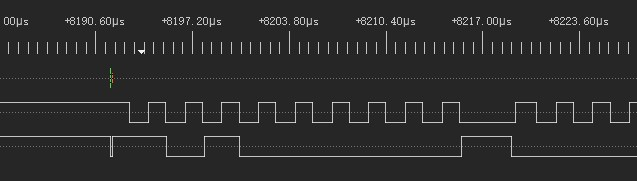
\includegraphics{q2_singal.jpg}
    \caption{第一步}
\end{figure}

问题Q3: 在读时不支持: 在不stop的情况下start
\begin{figure}[h]
    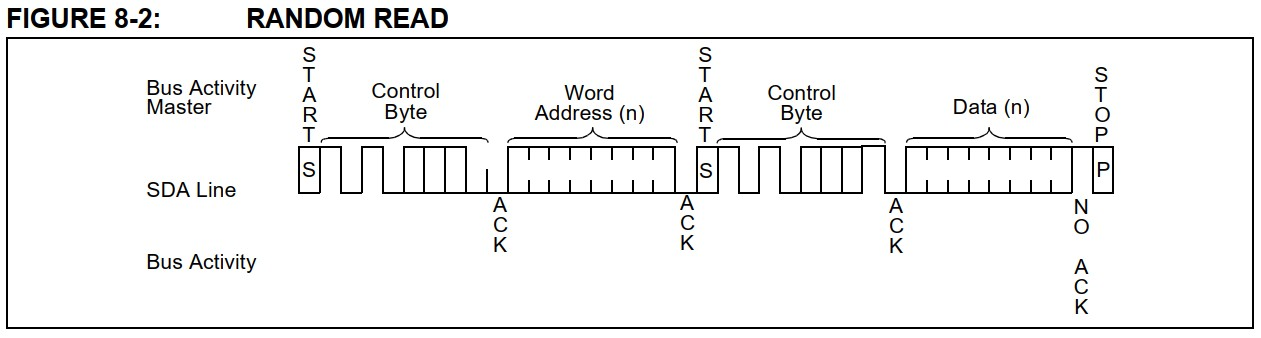
\includegraphics{eeprom_random_read.jpg}
    \caption{第一步}
\end{figure}



